\documentclass[tikz,border=8pt]{standalone}
\usepackage[scaled=0.95]{helvet}
\renewcommand{\familydefault}{\sfdefault}
\usepackage[europeanresistors,americanvoltages]{circuitikz}
\definecolor{TEJNavy}{HTML}{1E2B55}
\definecolor{TEJBlue}{HTML}{1769AA}
\begin{document}
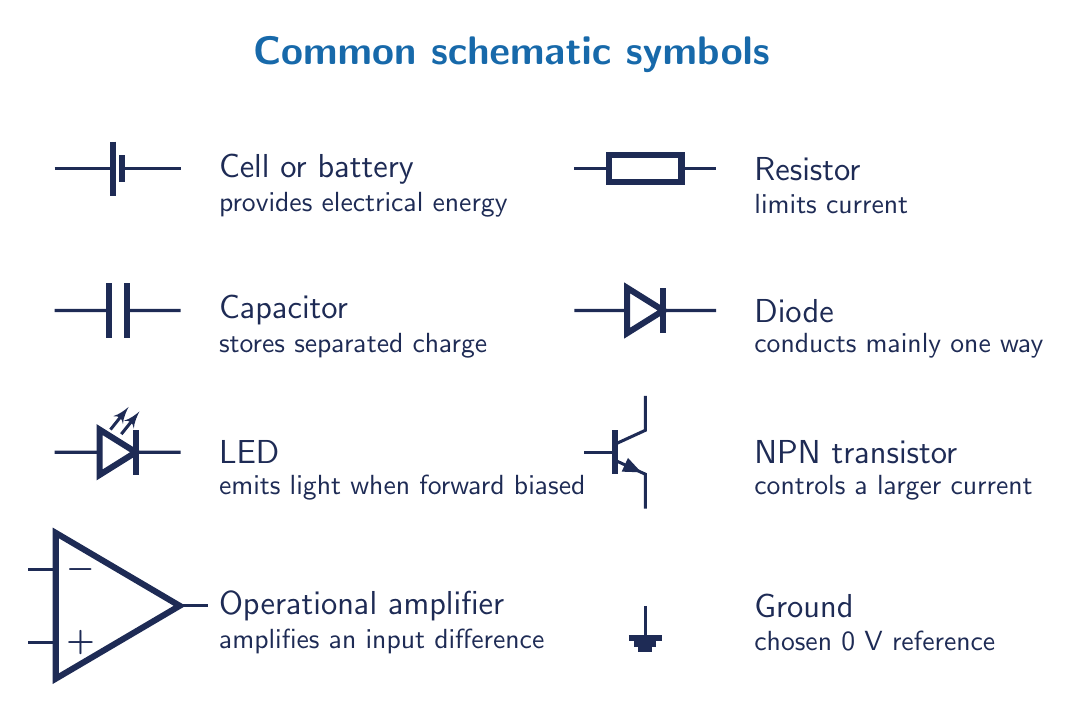
\begin{tikzpicture}[line width=1.1pt,draw=TEJNavy,text=TEJNavy,font=\sffamily]
  \ctikzset{bipoles/length=1.15cm}

  \node[font=\bfseries\Large,text=TEJBlue] at (6.2,7.35)
    {Common schematic symbols};

  \draw (0.4,5.9) to[battery1] (2.0,5.9);
  \node[anchor=west,font=\large] at (2.35,5.9) {Cell or battery};
  \node[anchor=west] at (2.35,5.45) {provides electrical energy};

  \draw (7.0,5.9) to[R] (8.8,5.9);
  \node[anchor=west,font=\large] at (9.15,5.9) {Resistor};
  \node[anchor=west] at (9.15,5.45) {limits current};

  \draw (0.4,4.1) to[C] (2.0,4.1);
  \node[anchor=west,font=\large] at (2.35,4.1) {Capacitor};
  \node[anchor=west] at (2.35,3.65) {stores separated charge};

  \draw (7.0,4.1) to[D] (8.8,4.1);
  \node[anchor=west,font=\large] at (9.15,4.1) {Diode};
  \node[anchor=west] at (9.15,3.65) {conducts mainly one way};

  \draw (0.4,2.3) to[leD] (2.0,2.3);
  \node[anchor=west,font=\large] at (2.35,2.3) {LED};
  \node[anchor=west] at (2.35,1.85) {emits light when forward biased};

  \node[npn,scale=1.1] at (7.9,2.3) {};
  \node[anchor=west,font=\large] at (9.15,2.3) {NPN transistor};
  \node[anchor=west] at (9.15,1.85) {controls a larger current};

  \node[op amp,scale=1.15] at (1.2,0.35) {};
  \node[anchor=west,font=\large] at (2.35,0.35) {Operational amplifier};
  \node[anchor=west] at (2.35,-0.10) {amplifies an input difference};

  \node[ground,scale=1.2] at (7.9,0.35) {};
  \node[anchor=west,font=\large] at (9.15,0.35) {Ground};
  \node[anchor=west] at (9.15,-0.10) {chosen 0 V reference};
\end{tikzpicture}
\end{document}
